\chapter{Scheduling CPU}
I processi vengono sempre eseguiti finché non richiedono di attendere un'altra risorsa.
A questo punto un sistema semplice attende la risorsa, sprecando cicli della CPU, con la multiprogrammazione puntiamo a ridurre i cicli sprecati al minimo.

\section{CPU scheduler}
Abbiamo visto in 2.3.1 il lifecycle di un processo, lo scheduler della CPU deve prendere una decisione in queste situazioni:
\begin{enumerate}
    \item \textbf{Suspend:} Avviene principalmente come risultato di una richiesta di I/O, è quindi richiesto dal processo stesso.
    \item \textbf{Resign:} Il processo viene forzatamente interrotto dallo scheduler.
    \item \textbf{Resume:} La condizione attesa diventa vera e il processo è pronto ad utilizzare nuovamente risorse di sistema.
    \item \textbf{Termina}
\end{enumerate}

Uno scheduler che effettua delle decisioni solo nel caso 1 e 4 si dice \textbf{senza diritto di prelazione}, il processo quindi viene eseguito fino al termine o finché non restituisce volontariamente il controllo al sistema operativo.

Gli scheduler dei sistemi operativi moderni sono tutti \textbf{con diritto di prelazione}, effettuano quindi tutte e 4 le decisioni per portare a migliori prestazioni.

\spacer
I kernel con diritto di prelazione devono gestire anche tutte le situazioni critiche:
\begin{sitemize}
    \item Possibili \textbf{Race condition} quando avviene l'accesso a dati condivisi tra processi.
    \item La possibilità che anche i processi del kernel vengano prelati interrompendo così operazioni cruciali effettuate dal sistema.
\end{sitemize}

\subsection{Implementazione}
Il massimo utilizzo delle risorse si ottiene implementando lo scheduler in modo tale che ogni processo esegua continui cicli di CPU-I/O burst.

\begin{figure}[H]
    \centering
    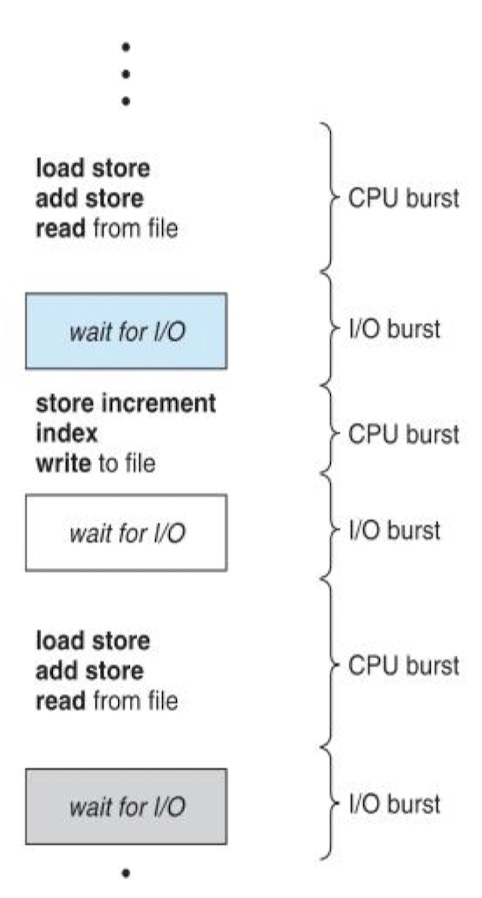
\includegraphics[width=0.22\linewidth]{assets/CPU-IO-burst.jpg}
\end{figure}

Ogni algoritmo di scheduling ha diversi criteri che prova ad ottimizzare, alcuni di questi sono:
\begin{sitemize}
    \item \textbf{Utilizzo della CPU}
    \item \textbf{Throughput:} Numero di processi che completano la loro esecuzione nell'unità di tempo.
    \item \textbf{Tempo di turnaround:} Tempo impiegato per l'esecuzione di un determinato processo
    \item \textbf{Tempo di attesa} nella ready queue
    \item \textbf{Tempo di risposta:} il tempo che intercorre tra una richiesta e una risposta.
\end{sitemize}

\begin{figure}[H]
    \centering
    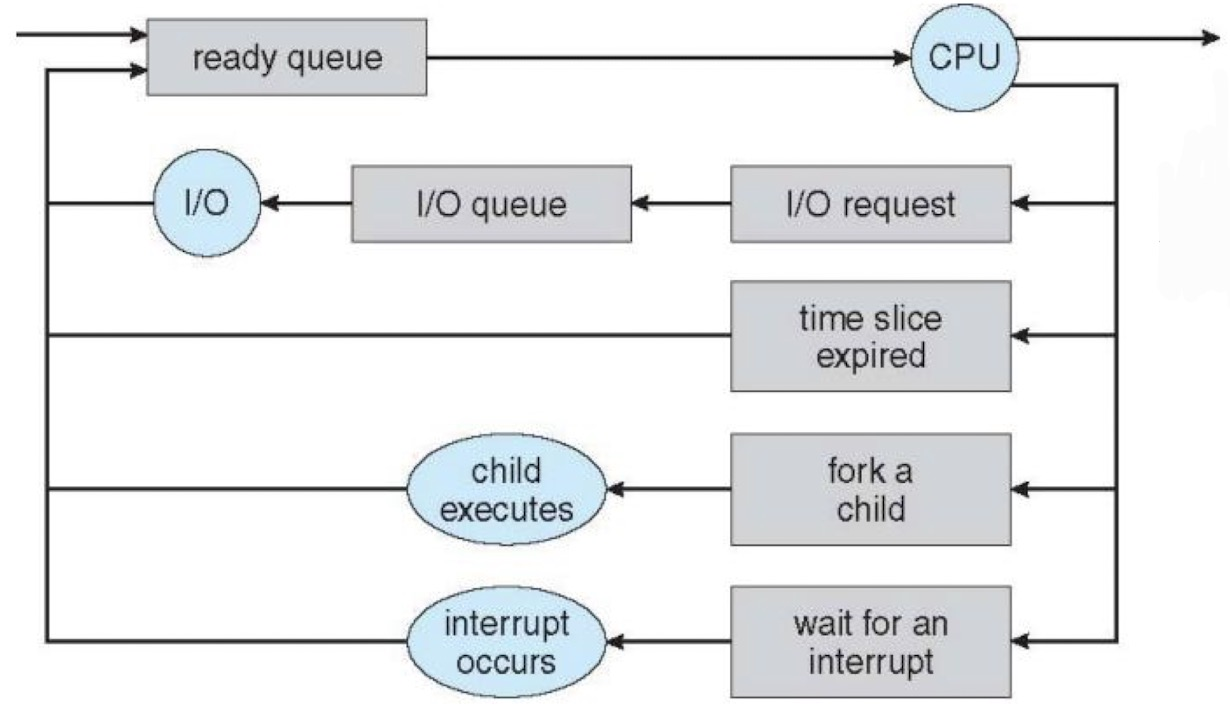
\includegraphics[width=0.5\linewidth]{assets/scheduler.jpg}
    \caption{Diagramma di scheduling}
\end{figure}

\subsection{Meccanismo di Interruzione}
Con \textbf{Meccanismo di Interruzione} intendiamo il meccanismo messo a disposizione dell'elaboratore per salvare lo stato del processo interrotto per poi trasferire il controllo ad una subroutine che gestisce l'interrupt.

\spacer
Il kernel del sistema è composto da 3 sezioni, il \textit{First Interrupt Handler (FLIH)}, il dispatcher e l'implementazione degli strumenti di sincronizzazione.

\subsubsection{First Interrupt Handler}
Il \textit{First Interrupt Handler (FLIH)} ha il compito di determinare l'origine dell'interrupt e attivare il segmento di codice che la gestisce.

\spacer
Nel caso di un sistema che implementa la multiprogrammazione ci possono essere più processi in attesa, è quindi necessario costruire una coda delle interruzioni.

La coda delle interruzioni funziona assieme a la coda dei processi pronti ad eseguire, quando un processo esce dalla coda delle interruzioni viene inserito tra gli altri processi pronti in attesa di risorse computazionali.

\begin{figure}[H]
    \centering
    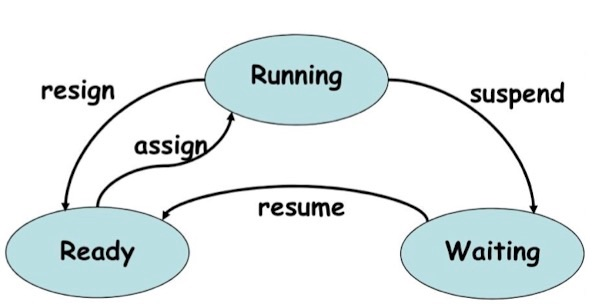
\includegraphics[width=0.45\linewidth]{assets/process-lifecycle.jpeg}
\end{figure}

\subsubsection{Implementazione Strumenti di Sincronizzazione}
Le primitive wait e signal sono implementate dal kernel in quanto possono essere utilizzate da tutti i processi, wait deve poter avere accesso diretto al dispatcher per comunicarci.

\spacer
Ogni semaforo ha una coda, in genere FIFO, che contiene tutti i processi che si sono fermati sul semaforo.

\begin{note}
    Non tutti i semafori sono implementati tramite FIFO, essi in generale possono avere diverse implementazioni e organizzazione.
\end{note}

\subsection{Dispatcher}
Il dispatcher ha il compito di assegnare le risorse di computazione al processo selezionato dallo scheduler. Esso gestisce il context switch tra vari processi.

\begin{figure}[H]
    \centering
    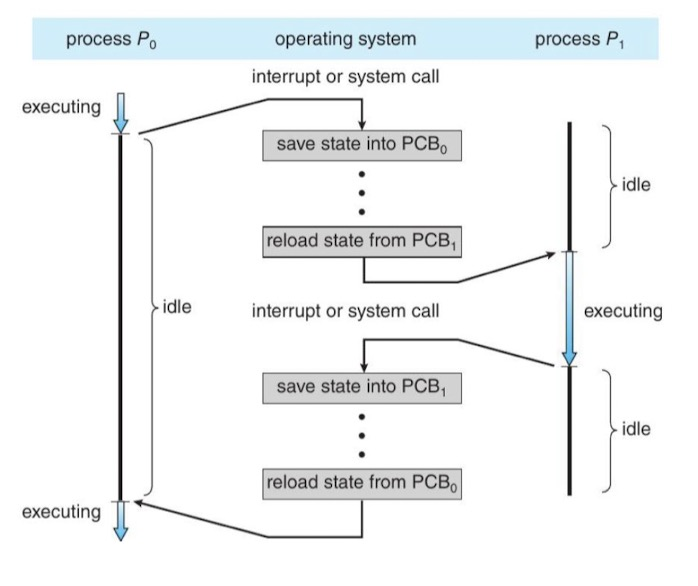
\includegraphics[width=0.5\linewidth]{assets/dispatcher.jpg}
    \caption{Context switch $P_0 \rightarrow P_1 \rightarrow P_0$ }
\end{figure}

Definiamo \textbf{Latenza di dispatch} il tempo impiegato dal dispatcher per scambiare un processo con un'altro. Nello schema qui sopra è il periodo in cui entrambi i processi sono in \textit{idle}.

\subsection{Scheduler ad alto livello}
Il compito di attrubuire il livello di priorità dei processi non è compito del dispatcher, ma dello scheduler di alto livello.

È possibile utilizzare un heap, così da avere buone prestazioni di inserzione ($O(\log_2 n)$) e rendere banale l'estrazione del processo a priorità maggiore.

\section{Comunicazione tra Processi}
La comunicazione tra processi è necessaria in diverse situazioni e viene implementata mediante diverse tecniche:
\begin{sitemize}
    \item \textbf{Scambio di Messaggi:} Richiede un overhead da parte del sistema operativo, ma non presenta conflitti ed è di più semplice utilizzo.
    \item \textbf{Memoria Condivisa:} Richiede l'intervento del kernel solo nell'allocazione iniziale, tuttavia gli accessi successivi devono essere gestiti direttamente dai processi.
    \item \textbf{Pipes Ordinarie:} Permettono la comunicazione unidirezionale tra due processi (produttore-consumatore).
    \item \textbf{Pipes Nominate:} Permettono la comunicazione bidirezionale a molteplici processi, questo avviene grazie ad un file di tipo speciale. Sono supportate sia da Unix che da Windows.
\end{sitemize}
\section{Algoritmi di Scheduling}

\subsection{Selezione}
Prima di vendere alcuni degli algoritmi più utilizzati dai sistemi operativi moderni vediamo il metodo che viene utilizzato per confrontare e migliorare gli algoritmi.

\subsubsection{Modelli Deterministici}
Nella valutazione analitica, si seleziona un set predeterminato di processi, e si simulano più algoritmi calcolandone il tempo medio di attesa nei vari casi.

\spacer
È possibile utilizzare la \textbf{Formula di Little} per avvicinarsi di più alla realtà:
Sia $n$ la lunghezza media della coda, $W$ il tempo medio di attesa e $\lambda$ il numero di processi in arrivo per unità di tempo. Allora $n = W \cdot \lambda$.

\subsubsection{Simulazione}
La simulazione implica la creazione di un modello del sistema di calcolo e un processo di logging dei dati.

\subsection{Algoritmi Comuni}

\subsubsection{First Come First Serve}
Un semplice algoritmo che fornisce le risorse al primo processo che le richiedono. Il criterio poi segue l'implementazione della coda FIFO, quando le risorse si liberano vengono assegnate al primo processo della coda.

Questa strategia non è efficace per i computer consumer in quanto un processo molto lungo può fermare l'esecuzione di altri processi brevi che l'utente richiede con maggiore urgenza.

\subsubsection{Highest Priority/Shortest Job First}
Viene fornito un valore di priorità ad ogni processo, le risorse vengono assegnate al processo con la priorità più alta.

Questo algoritmo presenta spesso il problema della \textit{starvation} dove i processi a priorità bassa non vengono mai eseguiti, ma introducendo l'\textit{aging} la priorità di un processo aumenta all'aumentare del suo tempo di attesa.

\subsubsection{Round Robin o Scheduling Circolare}
A ciascun processo vengono assegnate le risorse per un periodo di tempo limitato, solitamente 10-100 ms (un periodo più breve ha troppo overhead di switching, con uno più grande si ottiene un algoritmo FIFO)

Questo algoritmo ha in media un tempo medio di attesa maggiore di un algoritmo basato sulla priorità, ma ha un miglior tempo di risposta, cosa importante nei sistemi consumer.

\begin{figure}[H]
    \centering
    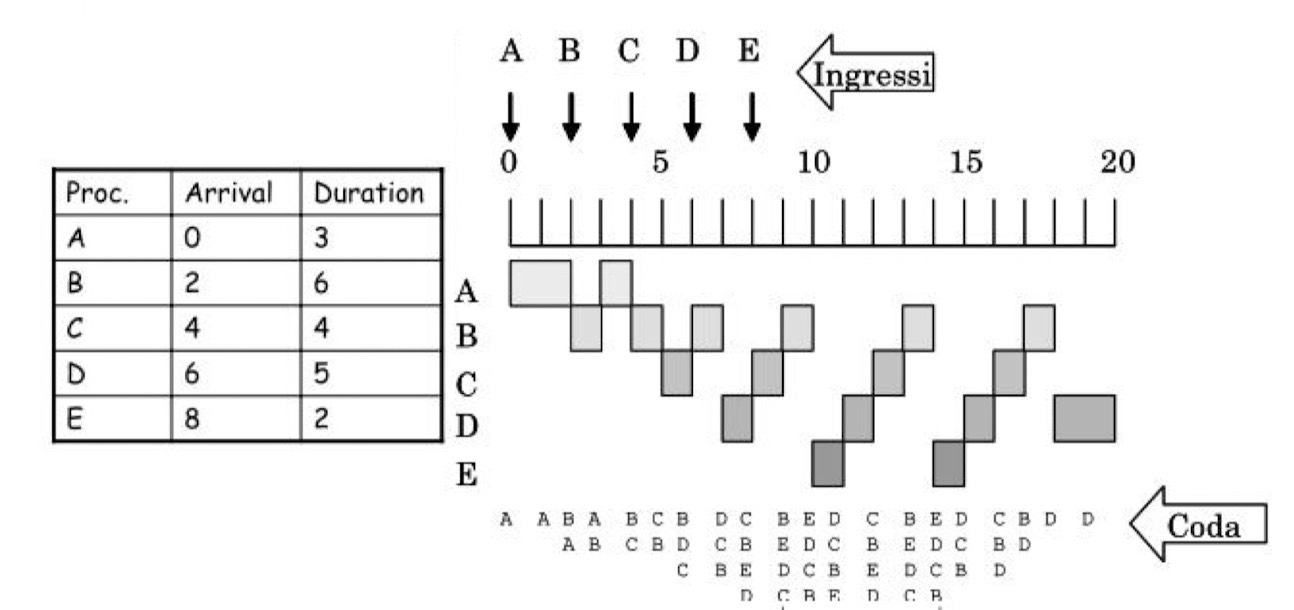
\includegraphics[width=0.65\linewidth]{assets/round-robin.jpg}
    \caption{Esempio di esecuzione dell'algoritmo}
\end{figure}

\begin{note}
    Spesso negli esercizi capita che un nuovo processo venga inserito nella coda ready allo stesso momento in cui un processo termina il suo quanto di tempo. Si incorre quindi in una situazione dove non è chiaro quale dei due processi verrà inserito prima nella ready queue.

    In questo caso è possibile scegliere la soluzione che si preferisce, con l'unico limite di restare consistenti all'interno dell'esercizio.
\end{note}

\subsubsection{Highest Response Ratio}
Definiamo un valore da utilizzare come priorità, la priorità del processo $P_i$ sarà $p_i = \frac{a_i + e_i}{e_i}$

Dove $a_i$ è il tempo di attesa del processo nello stato ready e $e_i$ è il tempo di esecuzione stimato.

\spacer
Questo significa che i processi brevi avranno una priorità maggiore, ma implementa anche l'\textit{aging} per evitare la \textit{starvation}.

\subsubsection{Code Multiple}
Come spesso accade la migliore soluzione vede l'utilizzo di più algoritmi allo stesso tempo, è possibile infatti costruire più code, tutte con algoritmi di gestione diversi. Poi sarà sufficiente allocare una certa percentuale di risorse ad ognuna delle code.

\subsubsection{Esempio 1.}
Questa strategia si può ad esempio utilizzare per dividere i processi che eseguono in foregorund e quelli in background. La coda in foreground avrà maggiore disponibilità di risorse e sarà gestita in Round Robin per assicurarsi un ottima esperienza utente, quella background avrà meno risorse a disposizione e sarà gestita in FIFO.

\subsubsection{Esempio 2.}
Le code multiple si possono utilizzare anche per implementare l'aging, ad esempio possiamo implementare 3 code nel seguente modo:

La prima e la seconda in Round Robin a 8 ms ed a 16 ms e l'ultima in FIFO.
In questo modo i processi ricevono tutti rapidamente 8 e poi 16 ms di tempo di esecuzione, risolvendo così i processi semplici, mentre i processi più lunghi finiscono nella coda FIFO e verranno eseguiti quando possibile.

\begin{figure}[H]
    \centering
    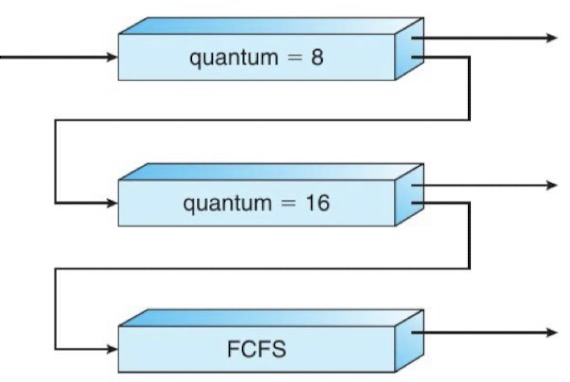
\includegraphics[width=0.32\linewidth]{assets/code-multiple.jpg}
\end{figure}

\subsubsection{Scheduling con Priorità Proporzionale alla frequenza}
Un caso tipico industriale è quello in cui i processi devono essere eseguiti ad intervalli regolari. In questo caso è conveniente definire una priorità proporzionale alla frequenza. Quindi processi che utilizzano la CPU con più frequenza avranno priorità maggiore.

\spacer
Questo è un algoritmo ottimale, quindi se esso non riesce a pianificare l'esecuzione di una serie di processi rispettando i vincoli temporali allora nessun altro algoritmo ci riuscirà.
\begin{figure}[H]
    \centering
    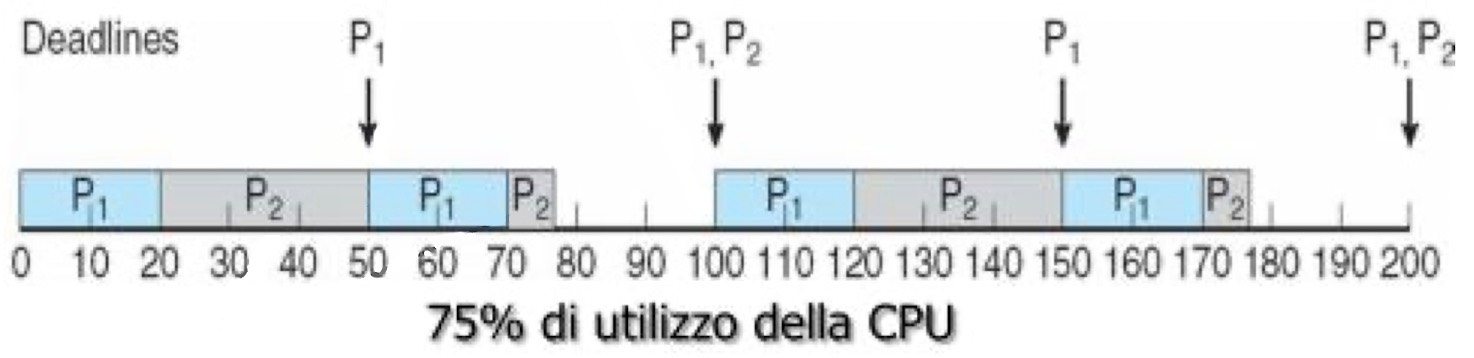
\includegraphics[width=0.6\linewidth]{assets/coda-frequenza.jpg}
\end{figure}

È possibile calcolare a priori se i processi potranno essere eseguiti rispettando i vincoli tramite la seguente formula:
$$\sum_{i=1}^{m}\frac{C_i}{P_i} \le m\cdot(2^{\frac{1}{m}} - 1)$$
dove m è il numero di processi $P_i$ il periodo del processo $i$ e $C_i$ la sua durata.

\subsubsection{Earliest Deadline First}
Assegna le priorità dinamicamente a seconda delle scadenze. Ogni processo per poter essere eseguito deve annunciare la sua prossima scadenza allo scheduler, più questa scadenza si avvicina più la priorità del processo aumenta.

\subsubsection{Esempio}
Siano due processi $P_1$ e $P_2$ con periodo di 50 e 80 e con tempo di esecuzione di 25 e 35.
\begin{figure}[H]
    \centering
    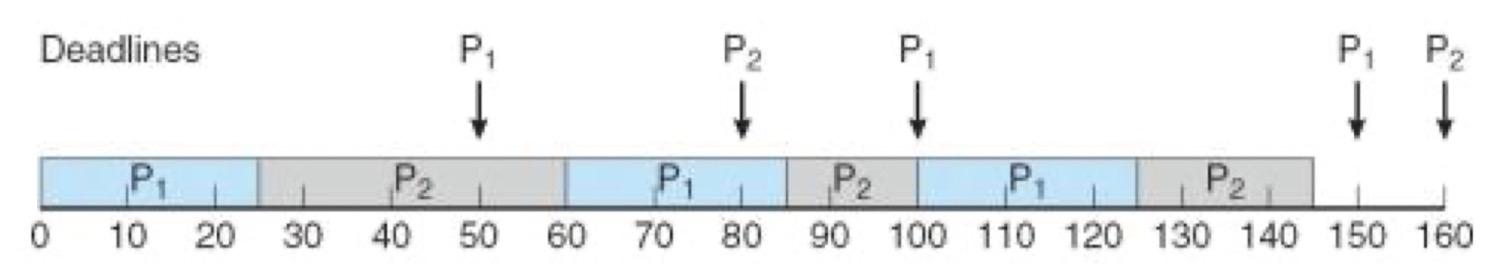
\includegraphics[width=0.6\linewidth]{assets/edf.jpg}
\end{figure}
Dalla figura si può vedere come a t=100 il processo $P_1$ interrompe $P_2$ in quanto la sua deadline è a t=150 mentre $P_2$ ha come deadline t=160

\section{Scheduling Multiprocessore}
Il problema dello scheduling diventa più complesso quando nel sistema di calcolo sono presenti più processori.

\subsubsection*{Multielaborazione asimmetrica}
Un singolo processore, detto \textit{master server} ha il compito di gestire lo scheduling, l'I/O e le altre attività di sistema.

Questo riduce la necessità di condividere dati, un solo processore deve accedere alle strutture dati.

\subsubsection*{Multielaborazione simmetrica}
Quando più processori lavorano su strutture dati comuni è possibile incorrere in delle situazioni critiche, ad esempio quando due processori non possono eseguire lo stesso processo e nessun processo deve subire \textit{starvation}.

\spacer
Ci sono due filosofie sull'implementazione di questo tipo di scheduling:
\begin{itemize}
    \item Una coda per ogni processore, questo ha problemi quando è necessario ribilanciare le code in quanto l'overhead in questo caso è significativo.
          \begin{figure}[H]
              \centering
              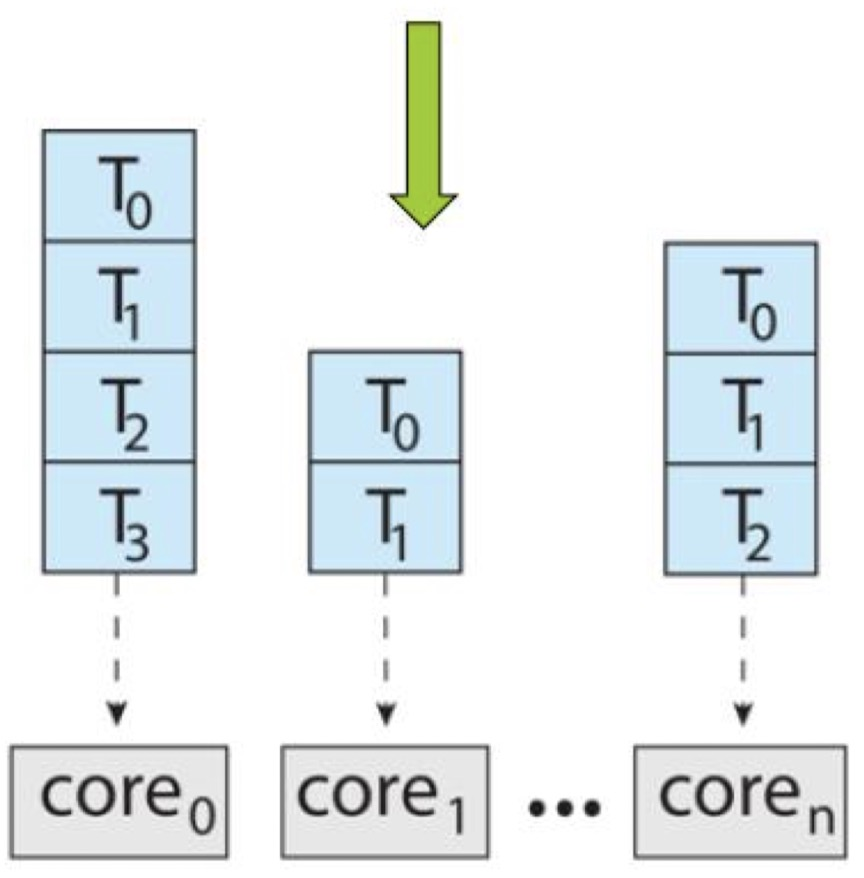
\includegraphics[width=0.3\linewidth]{assets/one-queue-one-core.jpg}
          \end{figure}

          \begin{note}
              In questo caso risulta essere importante ripartire uniformemente il carico tra i vari processori.

              Un controllo delle lunghezze delle code avviene sia periodicamente sia quando un determinato processore diventa inattivo.
          \end{note}

    \item Una singola coda per tutti i processori, questo risolve il problema del bilanciamento, ma genera delle race condition nell'accesso alla struttura dati.
          \begin{figure}[H]
              \centering
              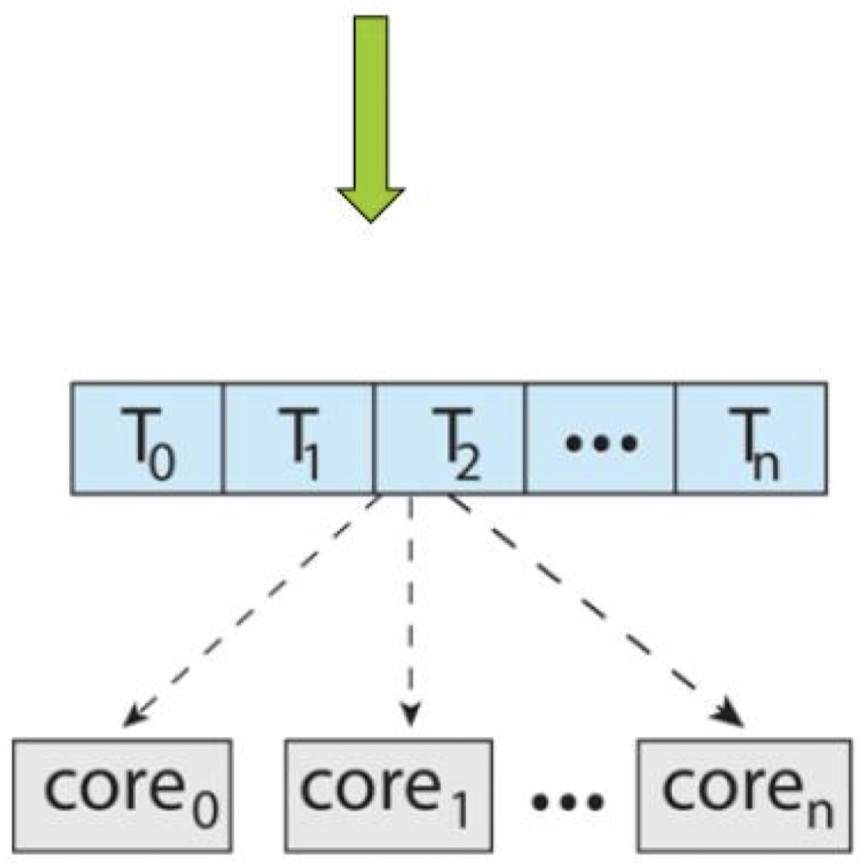
\includegraphics[width=0.3\linewidth]{assets/one-queue-many-core.jpg}
          \end{figure}
\end{itemize}

Esistono alcuni processi che hanno una predilezione per essere eseguiti sempre nello stesso core, questo permette loro di sfruttare al meglio la cache, ma non è sempre supportata dal sistema operativo.

\subsubsection*{Bilanciamento del Carico}
È il procedimento che permette di ripartire uniformemente il carico di lavoro tra più processori, può essere implementata in due modi:
\begin{sitemize}
    \item \textbf{Migrazione Guidata:} Un processo dedica controlla periodicamente il carico dei processori per correggere anticipamente gli equilibri
    \item \textbf{Migrazione Spontanea:} Un processore inattivo sottrae ad uno sovraccaricato un processo tra quelli in attesa.
\end{sitemize}

\subsection{Implementazioni}
\subsubsection{Linux}
Prima della versione 2.5 il kernel Linux implementava delle code multiple gestite perlopiù in Round Robin. La priorità viene calcolata periodicamente in base a quante risorse un processo ha consumato dall'ultimo controllo, minori sono le risorse utilizzate, maggiore sarà la priorità.

\spacer
Dalla versione 2.6.23 il kernel Linux implementa due code, \textit{default} e \textit{real-time}, con uno scheduler \textit{CFS (Completely Fair Scheduler)} che assegna ad ogni task una percentuale del tempo di CPU.

A ciascuna task viene associata una priorità (-20 a +19)

\spacer
Lo scheduler associa ad ogni task il suo tempo di esecuzione virtuale, una quantità che tiene conto sia del tempo di esecuzione che della priorità della task. Quindi una task a bassa priorità avrà un \texttt{vruntime} maggiore di una a priorità più alta, anche se sono state entrambe eseguite per lo stesso tempo.
Lo scheduler poi esegue la task con il valore \texttt{vruntime} più basso.

\spacer
Lo scheduler Linux è ottimizzato anche per sistemi NUMA, implementando delle strategie per ridurre al minimo il numero di migrazione dei processi da un processore all'altro.

\spacer
Le CPU Alder Lake causano non pochi problemi allo scheduler Linux < 5.16, infatti esso non si aspetta di vedere processori con livelli di prestazione diversi, ottimizzati per diverse situazioni.

\subsubsection{Windows 10}
Implementa livelli di priorità da 0 a 31, ognuno con la sua coda. Lo scheduler poi seleziona l'ultimo processo dalla coda a priorità più alta non vuota.

\spacer
I thread che hanno una priorità compresa tra 0 e 15 vengono gestiti dinamicamente, quando uno di essi viene portato in foreground, oppure riceve un input dall'utente, la sua priorità viene aumentata.

Inoltre la priorità dinamica viene diminuita di un livello ogni volta che il processo accede alle risorse della CPU, fino a tornare alla priorità base.

\subsubsection{Windows 11}
Windows 11 è stato scritto pensando alle nuove CPU intel, le quali hanno dei core ad alte prestazioni e degli altri ad alta efficienza.

Lo scheduler del sistema interagisce attivamente con un microcontrollore integrato nella CPU, chiamato \textit{Thread Director}.

Esso comunica al sistema operativo dei consigli sulla gestione dei processi processi prendendo in considerazione la situazione attuale del processore.

\spacer
Un'altra funzionalità introdotta da Windows 11 è il GPU accelerated scheduler, esso permette alla GPU di autogestire alcune task e la sua VRAM, alleggerendo il carico sulla CPU.

\subsubsection{Sistemi Real Time}
I sistemi operativi real time si dividono in:
\begin{sitemize}
    \item \textbf{Hard Real Time:} Richiedono il completamento di alcuni processi critici entro limiti specifici.
    \item \textbf{Soft Real Time:} Richiedono solo che ad alcuni processi venga fornita una priorità maggiore.
\end{sitemize}

